
\section{Torsionspendel}
In dem zweiten Versuch wurde mit einem Torsionspendel der Schubmodul sowie die Rückstellkraft des Drahtes berechnet.
Im Abgleich mit Literaturwerten wird dann die Behauptung %TODO gestützt oder verworfen
gestützt, dass der Draht aus Stahl besteht.
Zur Messung werden eine rotierende Scheibe, sowie eine Hantel mit verstellbaren Gewichten genutzt.
%TODO Ergebnis

\subsection{Methoden}
Das Torsionspendel bestand aus einem dünnen Draht, welches fest an einer Halterung angebracht war.
Am unteren Ende des Drahtes konnten durch einen Schraubmechanismus eine massive Metallscheibe und eine Hantel mit abnehmbaren und auf der Achse verschiebbaren Gewichtsscheiben angebracht werden.
Dabei dienten Kerben in der Achse dazu, die Gewichte in festen Abständen vom Mittelpunkt zu fixieren.
Zudem konnten die Gewichte komplett von der Hantelachse entfernt werden.
Es wurden nun die Zeiten über jeweils mehrere Schweingungsperioden gemessen.

Für die analoge Zeitmessung wird eine Unsicherheit von $u(T) = \frac{\SI{0,1}{\second}}{2\sqrt{6}}\approx \SI{20}{\milli\second}$ angenommen.
Da die Scheibe eine kleine Markierung hatte, konnte die Zeit gut anhand der Ruhelage abgeschätzt werden.
Dabei wurde die Ruhelage durch einen Stab hinter der Scheibe bzw. der Hantel markiert.

Der Draht hatte eine Länge von \SI{181}{\centi\meter}.
Da das Maßband sich ein wenig gebogen hat, kann hier eine Unsicherheit von $u(L) = \frac{\SI{5}{\milli\meter}}{2\sqrt6}\approx \SI{1,0}{\milli\meter}$ angenommen werden.
Für alle weiteren Längenmessungen mit dem Maßband kann der Wert besser abgelesen werden und es sei $u(R_z) = \frac{\SI{1}{\milli\meter}}{2\sqrt{6}}$.

Um sicher zu gehen, dass der Draht überall die gleiche Dicke aufweist, wurde dieser an fünf verschiedenen Stellen jeweils drei mal gemessen.
Der erste gemessene Wert war hierbei stets größer als die nachfolgenden, was auf eine Deformation des Drahtes beim messen hindeutet.
Aufgrund dieser erheblichen Deformation von bis zu $20\%$ wird im folgenden nur der erste Wert jeder Messung betrachtet.
Alle Werte der jeweils ersten Messung liegen nah beieinander und der Draht kann als gleichmäßig dick angesehen werden mit $R = \SI{0,25 +- 0,05}{\milli\meter}$.

\subsection{Datenauswertung}

\subsubsection*{Rotationsscheibe}
Es wurden neun Schwingungsperioden gemessen.
Damit ergibt sich eine Schwingungsdauer von \SI{33,00 +- 0,00}{\second}\footnote{Genauere Werte finden sich im Anhang in Tab. \ref{tab:schwingungsperioden}}.
Die Scheibe hat einen Durchmesser von \SI{15}{\centi\meter} und ein Gewicht von \SI{2,648}{\kilogram}.
Nach Gl. (34)
\begin{equation}
	G = \frac{4\pi L m_z R_z^2}{R^4 T^2}
\end{equation}
ist der Schubmodul gegeben mit $G = \SI{7,26+-0,26}{\giga\pascal}$\footnote{Für Unsicherheitsrechnungen siehe Anhang Gl. (\ref{eq:G-unc})}.

\subsubsection*{Hantel}
Es wurden für jede Konfiguration drei Schwingungsperioden gemessen.
Trägt man wie in Abb. \ref{fig:hantel-fit} dargestellt $T^2$ gegen $2 \, m_2 \, a^2$ auf, so kann man einen linearen Zusammenhang erkennen.
Hierbei wurde die Konfiguration ohne Hantelscheiben noch nicht betrachtet.
Durch einen linearen Fit\footnote{Programm: SciDaVis; Algorithmus: kleinste Quadrate} kann die Steigung $m$ ermittelt und nach Gl. (43) 
\begin{equation}
	\label{eq:hantel-t2}
	T^2 = \frac{4\pi^2}{D^*} (J_1 + 2 J_2 + 2 m_2 a^2)
\end{equation}
folgt $m = \frac{4\pi}{D^*}$.
(Es sei zu bedenken, dass $m$ von der Einheit \si{\second\squared\per\kilogram\per\meter\squared} $=$ \si{\per\newton\per\meter} ist.)
Daraus folgt ein rücktreibendes Direktionsmoment von 
\begin{equation}
	D^* = \frac{4\pi}{m} \approx \SI{2,640+-0,002}{\newton\meter}.
\end{equation}

Das Trägheitsmoment $J_1$ der Hantelachse kann im Spezialfall $m_2 = 0$ sowie $J_2 = 0$ mit Gl. (\ref{eq:hantel-t2}) bestimmt werden.
Es folgt $J_1 = \frac{T^2 D^*}{4\pi^2} \approx \SI{11,74 +- 0,02}{\kilogram\meter\squared}$.

Formt man Gl. (\ref{eq:hantel-t2}) nach $J_2$ um, so ist für $a = 0$ und $T^2 = y_0$ aus Abb. \ref{fig:hantel-fit} das Trägheitsmoment einer Hantelscheibe gegeben mit
\begin{equation}
	J_2 = \frac{\frac{y_0 D^*}{4 \pi^2} - J_1}{2} \approx \SI{0,7176 +- 0,0121}{\kilogram\meter\squared}.
\end{equation}

\begin{figure}[ht]
	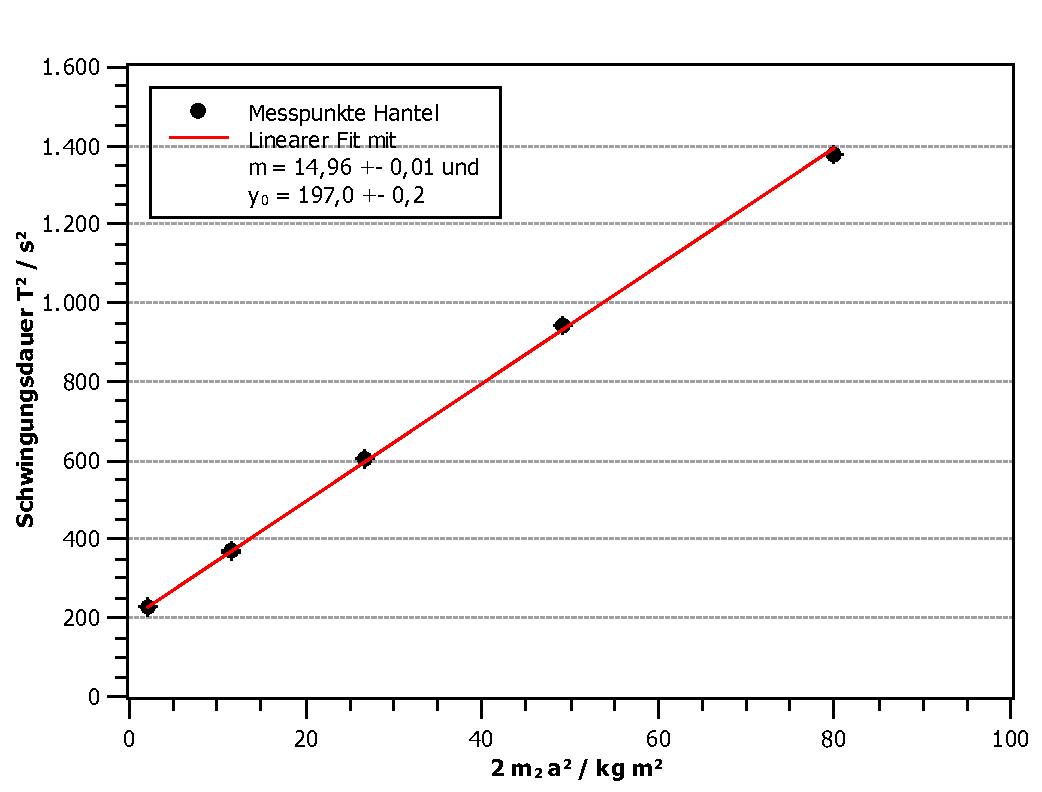
\includegraphics[width=\textwidth]{Torsion_Hantel_linear.pdf}
	\caption{Ausgleichsgerade durch linearisierte Messwerte.}
	\label{fig:hantel-fit}
\end{figure}

\subsection{Schlussfolgerung}
Durch die Messung eines Torsionspendels, konnte der Schubmodul für das Material des Drahtes auf $G = \SI{7,26+-0,26}{\giga\pascal}$ ermittelt werden.
%TODO Literaturwerte vergleichen und Quellen angeben
%TODO konnte die Hypothese bestätigt werden?
Um den Literaturwert genau zu überprüfen, muss die Dicke des Draht deutlich genauer gemessen werden.
Da der Schubmodul mit der vierten Potenz von dem Radius des Drahtes abhängt, muss eine Methode gefunden werden, welche die Mikrometerschraube stets mit der gleichen Kraft anzieht.
Zusätzlich sollte diese Kraft möglichst klein gehalten werden, um den Draht nicht beim messen zu deformieren.

\newpage

\section{Anhang}

\begin{table}[h]
	\centering
	\caption{Schwingungsdauer einer Periode. Bei der Hantel sind die Positionen der Gewichte von innen nach außen zu betrachten.}
	\label{tab:schwingungsperioden}
	\begin{tabular}{l|S}
		\hline
		{Scheibe} & \SI{32,996667 +-0,002268}{\second}\\
		{Hantel ohne Gewichte} & \SI{13,25+-0,006804}{\second}\\
		{Hantel 1. Position} & \SI{15,053333+-0,006804}{\second}\\
		{Hantel 2. Position} & \SI{19,19+-0,006804}{\second}\\
		{Hantel 3. Position} & \SI{24,573333+-0,006804}{\second}\\
		{Hantel 4. Position} & \SI{30,686667+-0,006804}{\second}\\
		{Hantel 5. Position} & \SI{37,136667+-0,006804}{\second}\\
		\hline
	\end{tabular}
\end{table}

\begin{figure}[h]
	\centering
	\begin{align}
	G =& \frac{4\pi L m_z R_z^2}{R^4 T^2}\\
	\begin{split}
		\label{eq:G-unc}
		u(G) =& \sqrt{\left( \pdv{G}{T} u(T) \right) ^2 + \left( \pdv{G}{L} u(L) \right) ^2 + \left( \pdv{G}{R_z} u(R_z) \right) ^2 + \left( \pdv{G}{R} u(R) \right) ^2}\\
		=& \frac{4\pi L m_z R_z^2}{R^4 T^2} \sqrt{\left(-\frac{2u(T)}{T} \right) ^2 + \left( \frac{u(L)}{L} \right) ^2 + \left( \frac{2u(R_z)}{R_z} \right) ^2 + \left( -\frac{4u(R)}{R} \right) ^2}\\
		\approx & \SI{13,015385}{\giga\pascal}
	\end{split}
	\end{align}
	\caption{Unsicherheitsrechnung für den Schubmodul des Drahtes mit der Torsionsschwingung der Scheibe.}
\end{figure}

\begin{figure}[h]
	\centering
	\begin{align}
		J_1 =& \frac{T^2 D^*}{4\pi^2}\\
		\begin{split}
			\label{eq:hantel-J1-unc}
			u(J_1) =& \sqrt{\left( \pdv{J_1}{T} u(T) \right) ^2 + \left( \pdv{J_1}{D^*} u(D^*) \right) ^2}\\
			=& \frac{T^2 D^*}{4\pi^2} \sqrt{\left( \frac{2 u(T)}{T} \right) ^2 + \left( \frac{u(D^*)}{D^*} \right)^2}\\
			\approx & \SI{0,015290}{\kilogram\meter\squared}
		\end{split}
	\end{align}
	\caption{Unsicherheitsrechnung für das Trägeitsmoment der Hantelachse ohne Gewichte.}
\end{figure}

\begin{figure}[h]
\centering
\begin{align}
J_2 =& \frac{\frac{y_0 D^*}{4 \pi^2} - J_1}{2}\\
\begin{split}
\label{eq:hantel-J2-unc}
u(J_2) =& \sqrt{\left( \pdv{J_2}{J_1} u(J_1) \right) ^2 + \left( \pdv{J_2}{D^*} u(D^*) \right) ^2 + \left( \pdv{J_2}{y_0} u(y_0) \right) ^2}\\
=& \frac{1}{2} \sqrt{\left( -u(J_1) \right) ^2 + \left( \frac{y_0}{4\pi^2} u(D^*) \right) ^2 + \left( \frac{D^*}{4\pi^2} u(y_0) \right) ^2}\\
\approx & \SI{0,010932637370106}{\kilogram\meter\squared}
\end{split}
\end{align}
\caption{Unsicherheitsrechnung für das Trägeitsmoment der Hantelgewichte.}
\end{figure}
